% \documentclass{beamer}
\documentclass[xcolor=dvipsnames]{beamer}
\usefonttheme{serif}
%% \usecolortheme[named=Blue]{structure}
\setbeamersize{text margin left=30mm, text margin right=30mm}
\useoutertheme{infolines}
%% \usetheme[height=7mm]{Rochester}
\usetheme{Pittsburgh}
\setbeamertemplate{items}[ball]
\setbeamertemplate{blocks}[rounded][shadow=true]
\setbeamertemplate{navigation symbols}{}

\usepackage[utf8x]{inputenc}
%% \usepackage{default}
\usepackage[english]{babel}
\usepackage{geometry}
%% \usepackage{fullpage}
\usepackage{amsmath, amsthm, amssymb}
\usepackage{listings}
\usepackage{pxfonts}
\usepackage{caption}

%% \usepackage{color}
%% \usepackage{graphicx}
%% \usepackage{natbib}
%% \usepackage{array}
%% \usepackage{booktabs}
%% \usepackage{tabu}
%% \usepackage[utf8]{inputenc}
%% \usepackage{fancyhdr}
%% \usepackage{float}
%% \usepackage{subfigure}
%% \usepackage{titlesec}

\setbeamertemplate{headline}{}
\setbeamertemplate{footline}[frame number]{}
\setbeamertemplate{navigation symbols}{}
\setbeamertemplate{footline}{}
\setbeamertemplate{footline}[frame number]


\def\CCT{{C\nolinebreak[4]\hspace{-.05em}\raisebox{.4ex}{\tiny\bf ++}}}
\def\CC{{C\nolinebreak[4]\hspace{-.05em}\raisebox{.4ex}{\small\bf ++}}}


\definecolor{lstgray}{gray}{0.93}
\definecolor{strgray}{gray}{0.4}

\lstset{ %
  escapechar=@,
  language=C++,
  basicstyle=\footnotesize\ttfamily,
  %% basicstyle=\ttfamily,
  %% keywordstyle=\color{blue}\ttfamily,
  keywordstyle=\bfseries,
  stringstyle=\color{strgray}\ttfamily,
  commentstyle=\color{OliveGreen}\ttfamily,
  %% morecomment=[l][\color{red}]{\#},
  morecomment=[l][\color{blue}]{\#},
  backgroundcolor=\color{lstgray},
  %% keywordstyle=\color{red},
  frame=f,
  frameround=ffff,
  tabsize=2,
  breaklines=true,
  breakatwhitespace=false,
  showspaces=false,
  showstringspaces=false,
  xleftmargin=5pt,
  xrightmargin=5pt,
  morekeywords={in,out,ref,auto,inout,import,ushort,scope,exit,mixin,decltype,varid,sizeof,constexpr}
}

\def\redcolor{\color{red}}
\def\bluecolor{\color{blue}}
\def\blackcolor{\color{black}}
\def\graycolor{\color{gray}}
\def\greencolor{\color{OliveGreen}}


\def\sectionname{\translate{Section}}
\def\insertsectionnumber{\arabic{section}}
\setbeamertemplate{section page}
{
  \begin{centering}
    \begin{beamercolorbox}[sep=4pt,center]{part title}
      \usebeamerfont{section title}\insertsection\par
    \end{beamercolorbox}
  \end{centering}
}
\def\sectionpage{\usebeamertemplate*{section page}}


\AtBeginSection{\frame{\sectionpage}}


\title{Compile time functions}
\subtitle{An introduction}
\author{Dominic Jones}
\date{\small{August 2018}}
\institute{\small{\texttt{github.com/DominicJones}}}


\begin{document}
\begin{frame}[plain]
  \titlepage
\end{frame}


\begin{frame}[fragile]{Compile time functions}
  \begin{enumerate}
  \item Like learning another language \vspace{5mm}
  \item Takes \emph{much} longer than writing its plain old equivalent \vspace{5mm}
  \item Worth taking time to \emph{play around} with implementation variations \vspace{5mm}
  \item Designing on paper saves a lot of grief! \vspace{5mm}
  \end{enumerate}
\end{frame}


\begin{frame}[plain]
  \begin{columns}[T] % align columns
    %% \begin{column}{0.3\textwidth}
    %% \end{column}%
    %% \hfill%
    \begin{column}{0.9\textwidth}
      \begin{figure}[H]
        \centering
        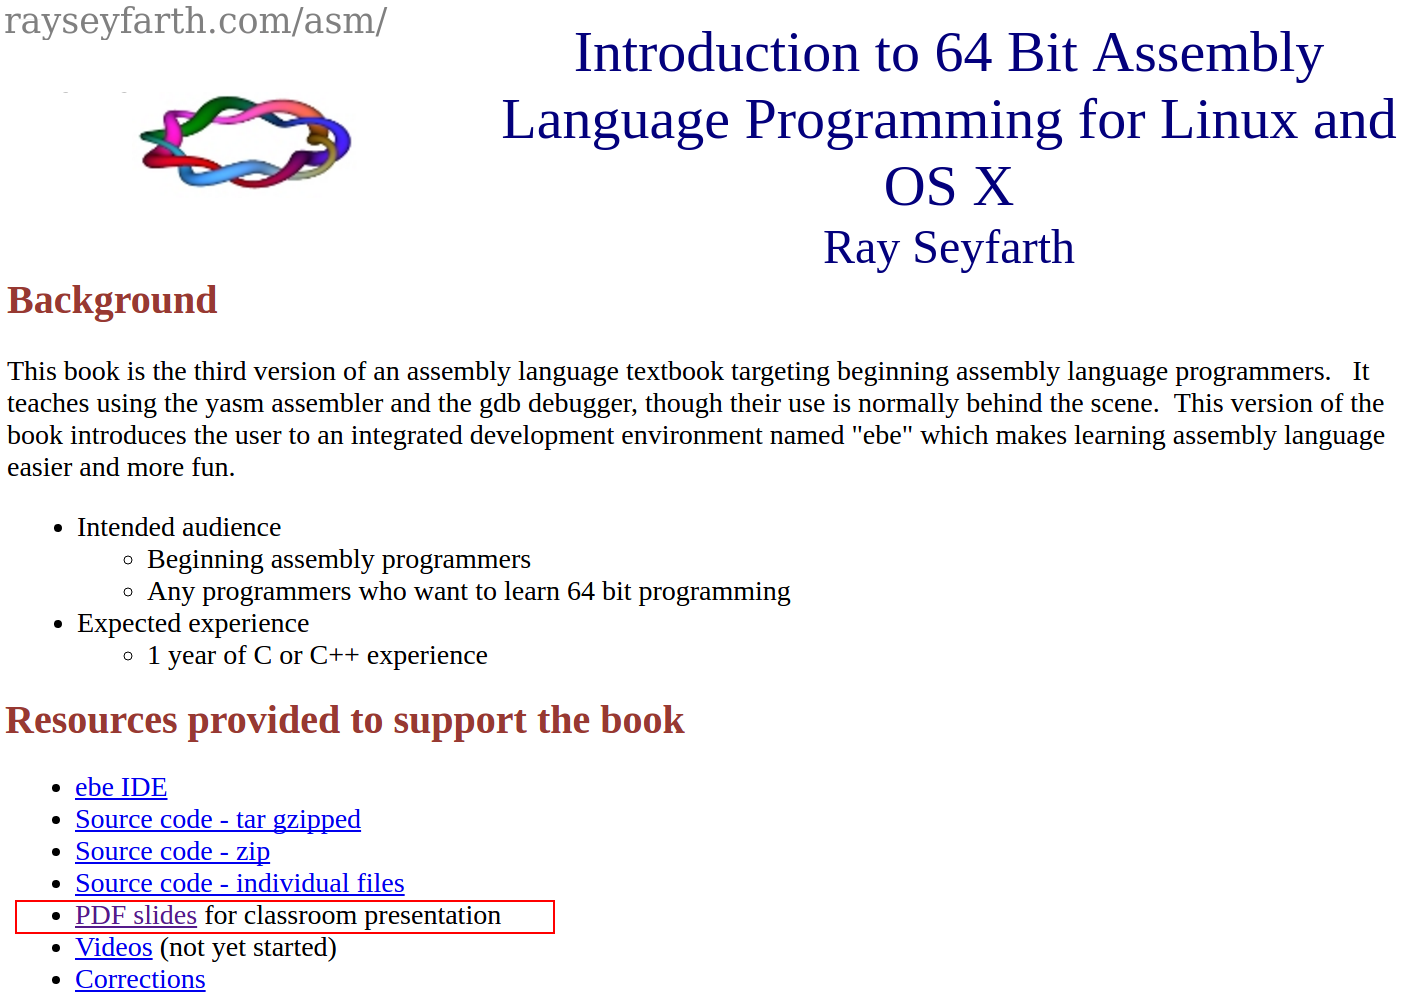
\includegraphics[width=0.99\textwidth]{ray_seyfarth}
      \end{figure}
    \end{column}%
  \end{columns}
\end{frame}


\begin{frame}[fragile]{An introduction}
  \begin{enumerate}
  \item The basics \vspace{5mm}
  \item Refactoring expressions \vspace{5mm}
  \item Functions as arguments \vspace{5mm}
  \item Cost of compilation \vspace{5mm}
  \item Mapping indices \vspace{5mm}
  \end{enumerate}
\end{frame}


\section{The basics}


\begin{frame}[fragile]{Zero or more}
\begin{lstlisting}
// no state, but instantiable
template<class... T> struct @\aftergroup\bluecolor@list@\aftergroup\blackcolor@ {};
\end{lstlisting}

~

\begin{lstlisting}
// a more useful form...
template<class T, T...> struct @\aftergroup\bluecolor@seq@\aftergroup\blackcolor@ {};
\end{lstlisting}

~

\begin{lstlisting}
// _the_ operation
template<class L> struct front;

template<template<class...> class L, class @\aftergroup\bluecolor@T1@\aftergroup\blackcolor@, class... T>
struct front<L<@\aftergroup\bluecolor@T1@\aftergroup\blackcolor@, T...> >
{
  using type = @\aftergroup\bluecolor@T1@\aftergroup\blackcolor@;
};
\end{lstlisting}
\end{frame}


\begin{frame}[plain]
  \begin{columns}[T] % align columns
    %% \begin{column}{0.3\textwidth}
    %% \end{column}%
    %% \hfill%
    \begin{column}{0.9\textwidth}
      \begin{figure}[H]
        \centering
        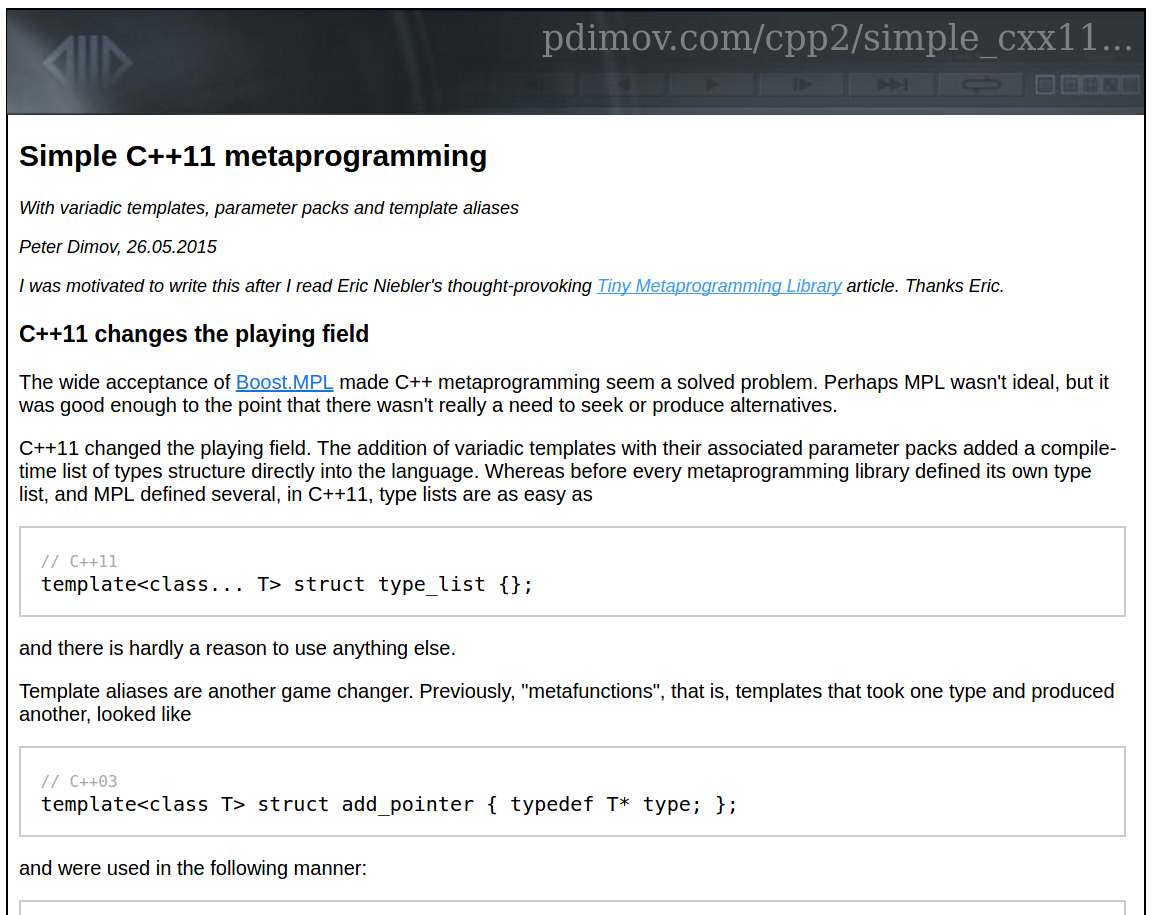
\includegraphics[width=0.99\textwidth]{pdimov}
      \end{figure}
    \end{column}%
  \end{columns}
\end{frame}


\section{Some not so obvious things}

\begin{frame}[fragile]{Incomplete types}
\begin{lstlisting}
// could be written as a class template...
template<class T> using @\aftergroup\bluecolor@add_pointer@\aftergroup\blackcolor@ = T*;
\end{lstlisting}

~

\begin{lstlisting}
// (to be revisited)
template<template<class... T> @\aftergroup\bluecolor@class F@\aftergroup\blackcolor@> struct bind;
\end{lstlisting}

~

\begin{lstlisting}
// `add_pointer' is unqualified
//  but still satisfies `bind'!
using incomplete_type = bind<@\aftergroup\bluecolor@add_pointer@\aftergroup\blackcolor@>;
\end{lstlisting}
\end{frame}


\begin{frame}[fragile]{Lazy construction}
\begin{lstlisting}
// nesting defers type construction
template<int N> struct @\aftergroup\bluecolor@lazy_seq@\aftergroup\blackcolor@
{
  using type = std::make_index_sequence<N>;
};
\end{lstlisting}

~

\begin{lstlisting}
// requiring additional `::type' wrapper
template<bool B, int NT, int NF>
using make_seq = std::conditional_t<B, @\aftergroup\bluecolor@lazy_seq@\aftergroup\blackcolor@<NT>,
                                       @\aftergroup\bluecolor@lazy_seq@\aftergroup\blackcolor@<NF> >;
\end{lstlisting}
\end{frame}


\begin{frame}[fragile]{Recursion}
\begin{lstlisting}
template<class... L> struct append;
\end{lstlisting}

~

\begin{lstlisting}
// join lists
template<template<class...> class L1, class... T1,
         template<class...> class L2, class... T2,
         class... L>
struct @\aftergroup\bluecolor@append@\aftergroup\blackcolor@<L1<T1...>, L2<T2...>, L...>
{
  using type = typename @\aftergroup\bluecolor@append@\aftergroup\blackcolor@<L1<T1..., T2...>, L...>::type;
};
\end{lstlisting}

~

\begin{lstlisting}
// ... until only one is left
template<template<class...> class L, class... T>
struct append<L<T...> >
{
  using type = L<T...>;
};
\end{lstlisting}
\end{frame}


\section{Refactoring expressions}


\begin{frame}[fragile]{Having and eating cake}
\begin{lstlisting}
// looks nice
r = (A + B)[i];
\end{lstlisting}

~

\begin{lstlisting}
// works well
r = A[i] + B[i];
\end{lstlisting}
\end{frame}


\begin{frame}[plain]
  \begin{columns}[T] % align columns
    %% \begin{column}{0.3\textwidth}
    %% \end{column}%
    %% \hfill%
    \begin{column}{0.8\textwidth}
      \begin{figure}[H]
        \centering
        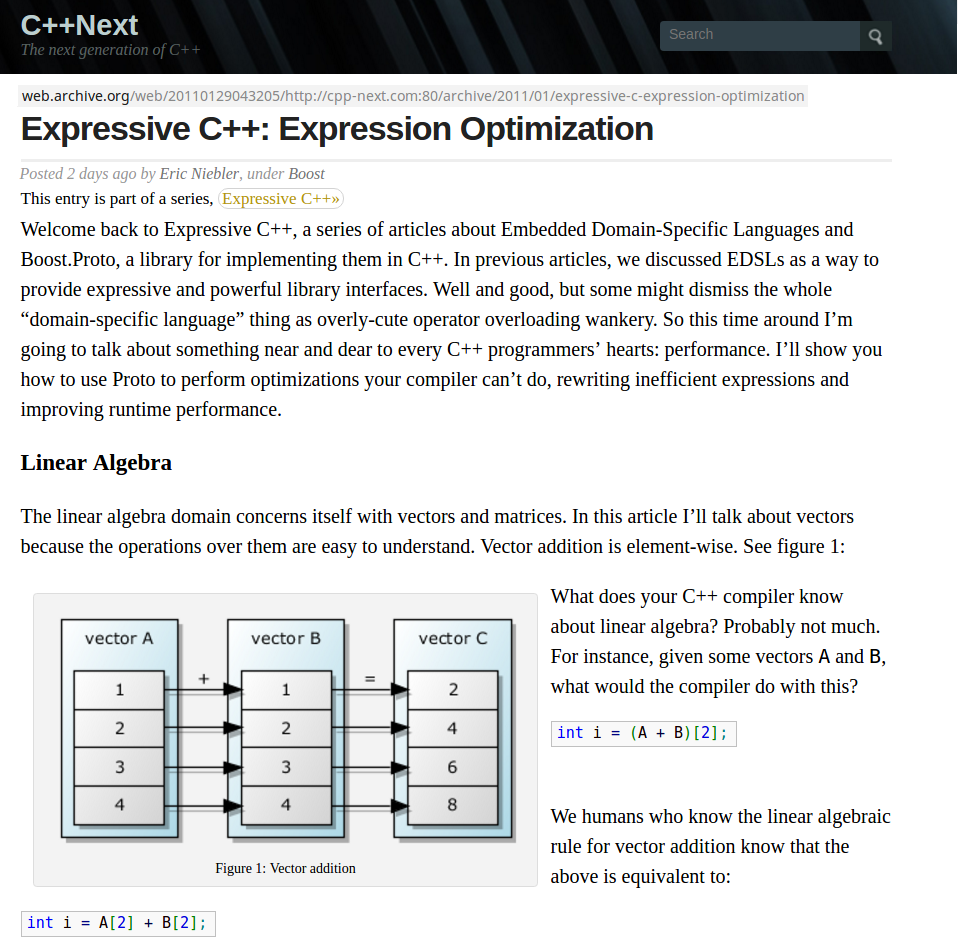
\includegraphics[width=0.99\textwidth]{niebler}
      \end{figure}
    \end{column}%
  \end{columns}
\end{frame}


\begin{frame}[fragile]{Having and eating cake}
  \begin{columns}[T] % align columns
    \begin{column}{0.35\textwidth}
      \begin{figure}[H]
        \centering
        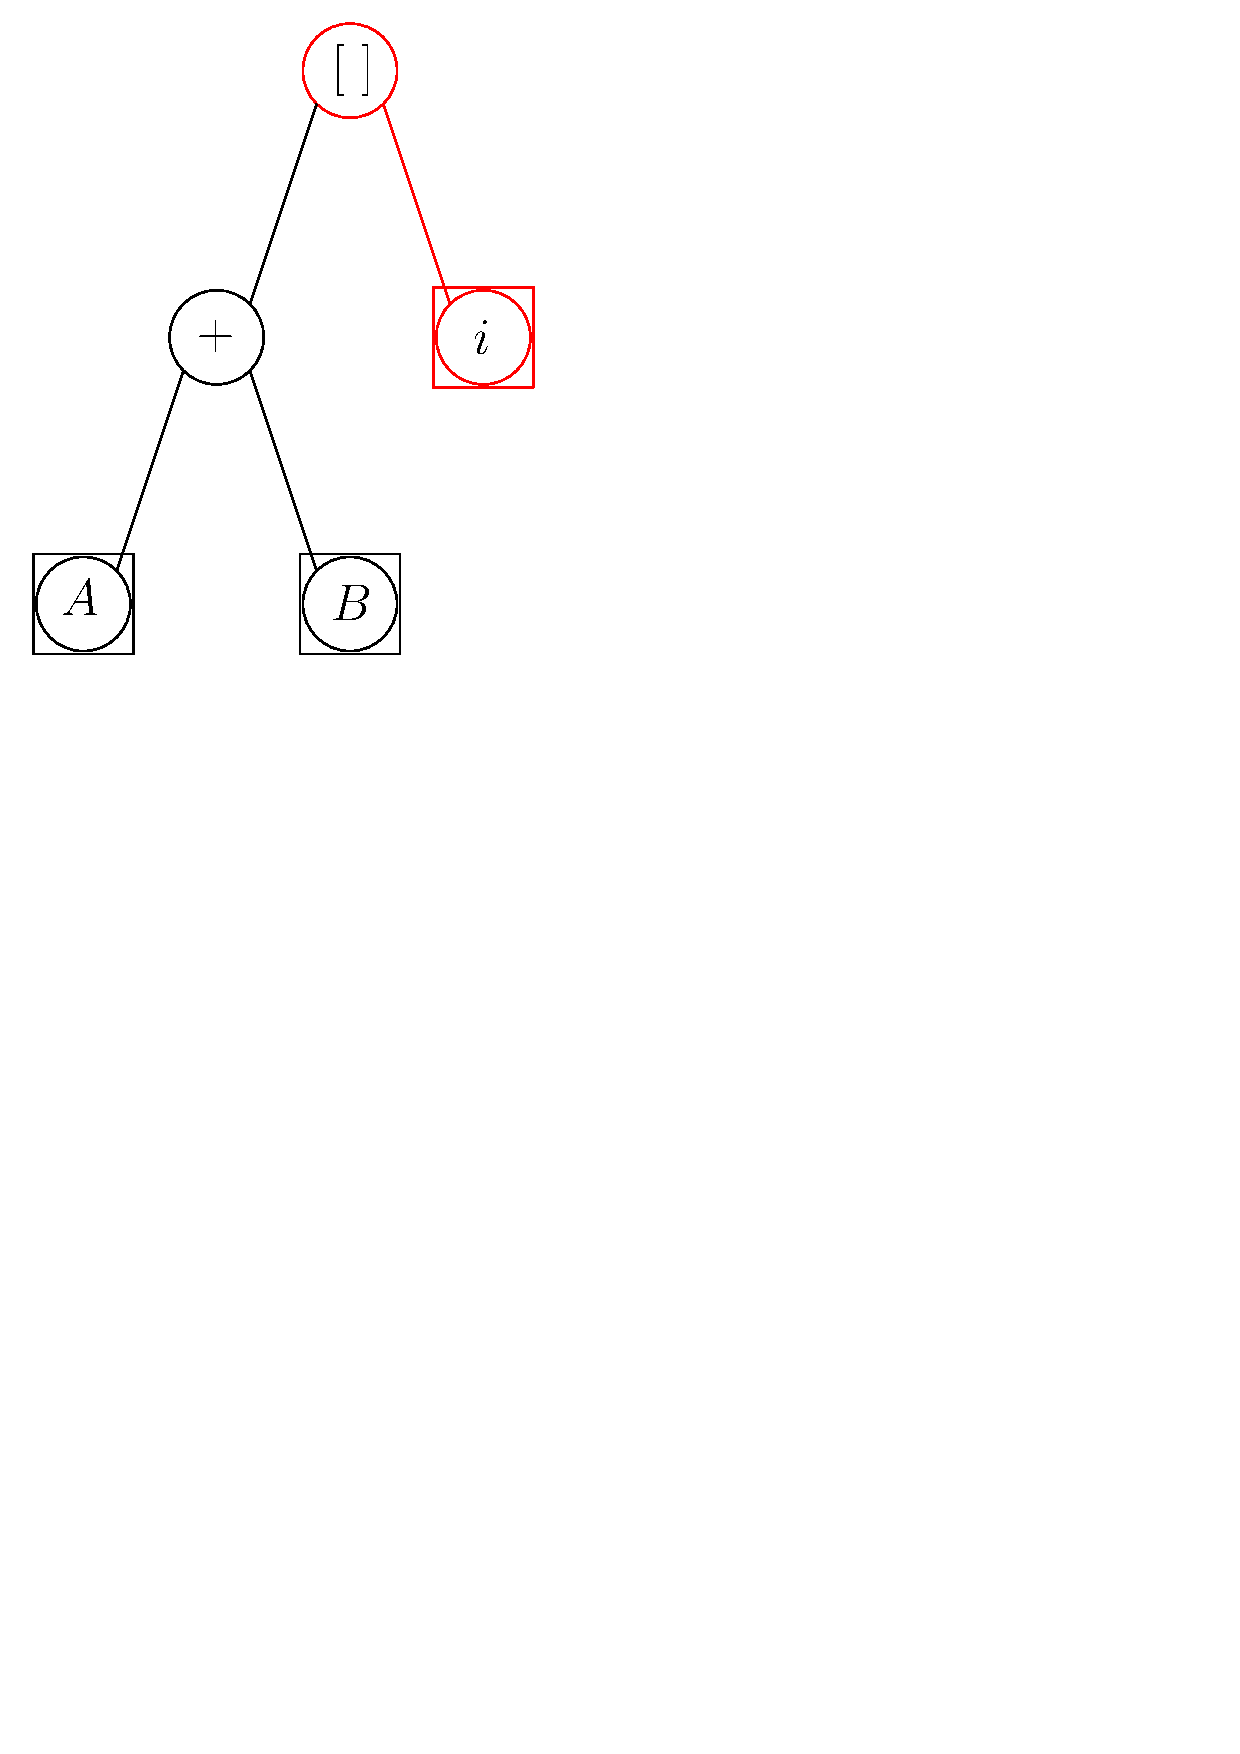
\includegraphics[width=4.3cm]{fig_expr_cb}
        \caption*{\texttt{(A + B)[i]}}
      \end{figure}
    \end{column}%
    \hfill%
    \begin{column}{0.55\textwidth}
      \begin{figure}[H]
        \centering
        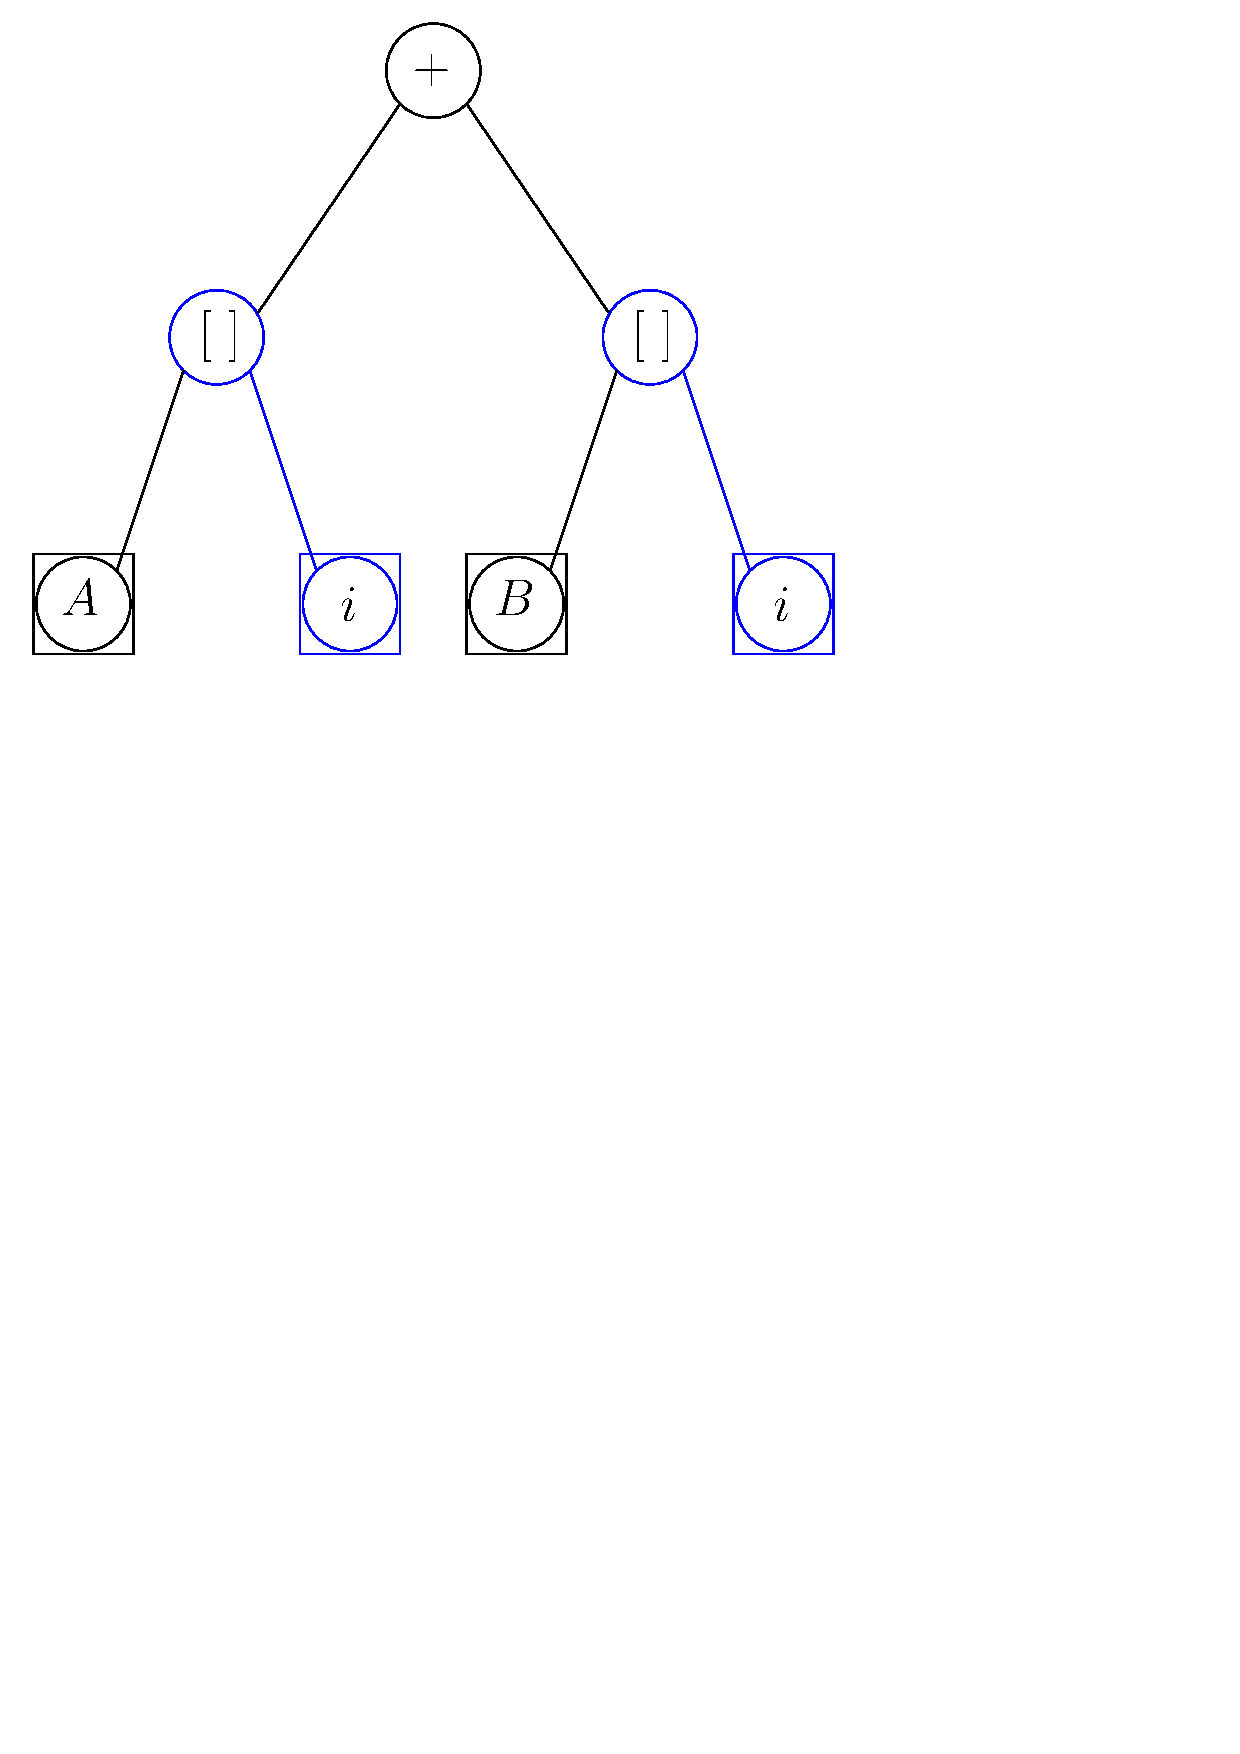
\includegraphics[width=7cm]{fig_expr_opt_cb}
        \caption*{\texttt{A[i] + B[i]}}
      \end{figure}
    \end{column}%
  \end{columns}
\end{frame}


\begin{frame}[fragile]{Having and eating cake}
\begin{lstlisting}
// (A + B)[i]
Binary<Idx, Binary<Add, A, B>, int>
\end{lstlisting}

~

\begin{lstlisting}
// apply special rules...
@\aftergroup\bluecolor@transform@\aftergroup\blackcolor@((A + B)[i])
\end{lstlisting}

~

\begin{lstlisting}
// A[i] + B[i]
Binary<Add, Binary<Idx, A, int>,
            Binary<Idx, B, int> >
\end{lstlisting}
\end{frame}


\begin{frame}[fragile]{Having and eating cake}
\begin{lstlisting}
// default transform: do nothing
template<class E> auto transform(E e)
{
  return e;
}
\end{lstlisting}
\end{frame}


\begin{frame}[fragile]{Having and eating cake}
\begin{lstlisting}
// push `Idx' operation down to the child nodes
template<class LF, class LL, class LR, class R>
auto transform(@\aftergroup\redcolor@Binary<Idx,@\aftergroup\blackcolor@ Binary<LF, LL, LR>, @\aftergroup\redcolor@R>@\aftergroup\blackcolor@ e)
{
  return
    transform(
      @\aftergroup\bluecolor@Binary<LF,@\aftergroup\blackcolor@ Binary<Idx, decltype(transform(e.l.l)), R>,
                 Binary<Idx, decltype(transform(e.l.r)), R> @\aftergroup\bluecolor@>@\aftergroup\blackcolor@
        {{transform(e.l.l), transform(e.r)},
         {transform(e.l.r), transform(e.r)}});
}
\end{lstlisting}
\end{frame}


\begin{frame}[fragile]{Having and eating cake}
\begin{lstlisting}
// apply transforms to child nodes
template<class F, class L, class R>
auto transform(Binary<F, L, R> e)
{
  return
    Binary<F, decltype(transform(e.l)),
              decltype(transform(e.r))>
      {transform(e.l), transform(e.r)};
}
\end{lstlisting}

~

\begin{lstlisting}
// needed for cases like:
@\aftergroup\bluecolor@transform@\aftergroup\blackcolor@(((A+B) - (C+D))[i])
\end{lstlisting}
\end{frame}


\section{Functions as arguments}


\begin{frame}[fragile]{Splitting things up}
  \begin{columns}[T] % align columns
    %% \begin{column}{0.3\textwidth}
    %% \end{column}%
    %% \hfill%
    \begin{column}{1.05\textwidth}
      \begin{figure}[H]
        \centering
        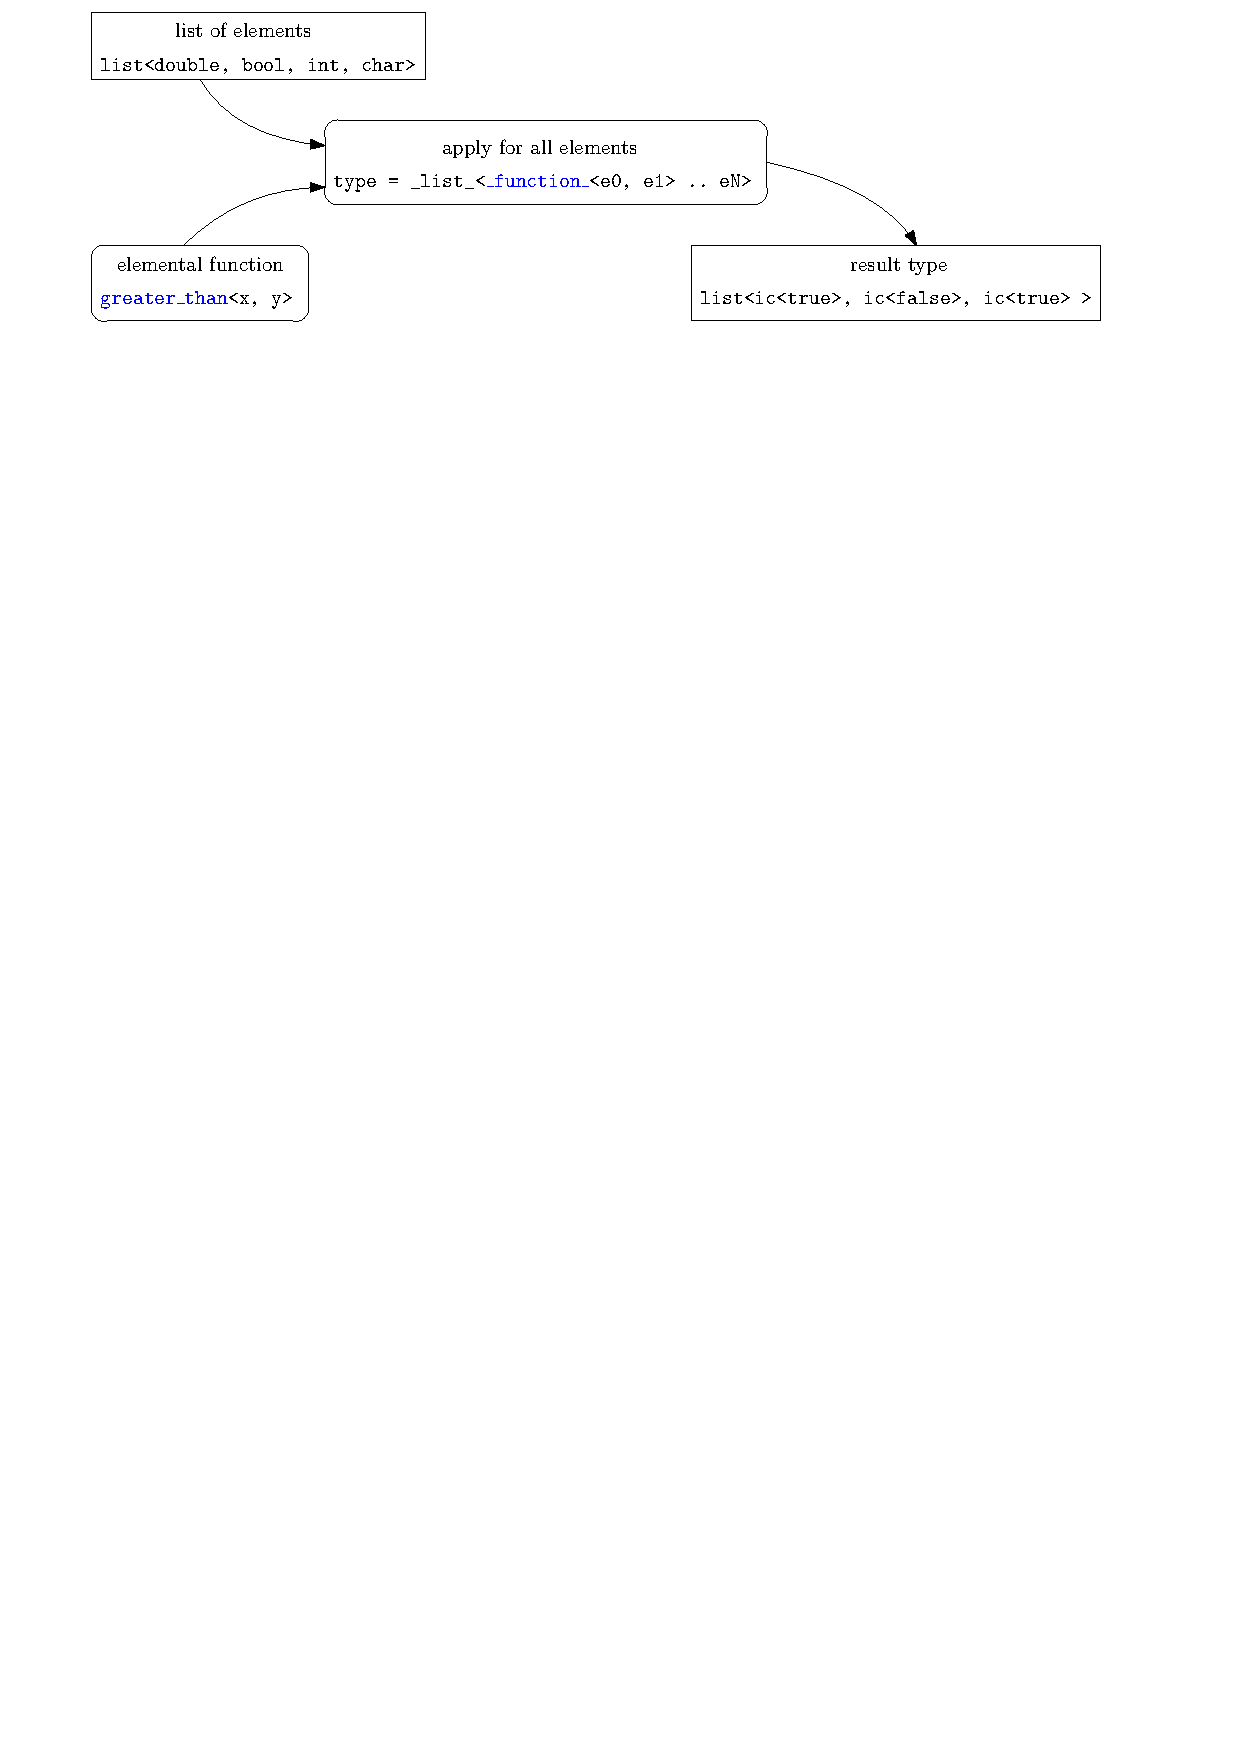
\includegraphics[width=0.99\textwidth]{second_order_func}
      \end{figure}
    \end{column}%
  \end{columns}
\end{frame}

\begin{frame}[fragile]{Splitting things up}
\begin{lstlisting}
struct @\aftergroup\bluecolor@_1@\aftergroup\blackcolor@;  struct @\aftergroup\bluecolor@_2@\aftergroup\blackcolor@;
template<template<class...> class, class...> struct bind;
\end{lstlisting}

\begin{lstlisting}
// apply
template<class L, class P> struct apply;

template<template<class...> class L, class T, class... Ts,
         template<class...> class F>
struct apply<L<T, Ts...>, bind<F, @\aftergroup\bluecolor@_1@\aftergroup\blackcolor@, @\aftergroup\bluecolor@_2@\aftergroup\blackcolor@> >
{
  using type = L<F<T, Ts>...>;
};
\end{lstlisting}
\begin{lstlisting}
// greater_than
template<class X, class Y>
using greater_than = bool_t<(sizeof(X) > sizeof(Y))>;
\end{lstlisting}

\begin{lstlisting}
// example
using L = list<int, bool, char, double>;
using R = apply_t<L, bind<greater_than, @\aftergroup\bluecolor@_1@\aftergroup\blackcolor@, @\aftergroup\bluecolor@_2@\aftergroup\blackcolor@> >;
\end{lstlisting}
\end{frame}


\begin{frame}[fragile]{Back to \texttt{bind}}
\begin{lstlisting}
// `unnamed' variables of a function signature
struct @\aftergroup\bluecolor@_1@\aftergroup\blackcolor@;  struct @\aftergroup\bluecolor@_2@\aftergroup\blackcolor@;
\end{lstlisting}

~

\begin{lstlisting}
// accepts a type of the form `F<T...>'
// and, optionally, some other types too
template<template<class...> class, @\aftergroup\bluecolor@class...@\aftergroup\blackcolor@> struct bind;
\end{lstlisting}
\end{frame}


\begin{frame}[fragile]{Leveraging incompleteness}
\begin{lstlisting}
// apply the transformation `P' to list `L'
template<class L, class P> struct apply;
\end{lstlisting}

~

\begin{lstlisting}
// the magic step:
//   `_1' and `_2' serve only to
//   match the class specialisation
template<template<class...> class L, class T, class... Ts,
         template<class...> class F>
struct apply<L<T, Ts...>, bind<F, @\aftergroup\bluecolor@_1@\aftergroup\blackcolor@, @\aftergroup\bluecolor@_2@\aftergroup\blackcolor@> >
{
  using type = L<F<T, Ts>...>;
};
\end{lstlisting}
\end{frame}


\begin{frame}[fragile]{\emph{The rub}}
\begin{lstlisting}
// `greater_than' must be forwarded to an `apply'
// specialised for two function variables
using R = apply_t<L, bind<greater_than, @\aftergroup\bluecolor@_1@\aftergroup\blackcolor@, @\aftergroup\bluecolor@_2@\aftergroup\blackcolor@> >;
\end{lstlisting}
\end{frame}


\section{Cost of compilation}


\begin{frame}[fragile]{Linear scaling}
\begin{lstlisting}
template<class S> struct concat;

template<int... I>
struct @\aftergroup\redcolor@concat@\aftergroup\blackcolor@<seq<I...> >
{
  using type = seq<0, (1 + I)...>;
};
\end{lstlisting}

\begin{lstlisting}
template<int N> struct make_seq;

template<> struct make_seq<0> { using type = seq<>; };

template<int N> struct @\aftergroup\bluecolor@make_seq@\aftergroup\blackcolor@
{
  using type = @\aftergroup\redcolor@concat_t@\aftergroup\blackcolor@<@\aftergroup\bluecolor@make_seq_t@\aftergroup\blackcolor@<(N-1)> >;
};
\end{lstlisting}

~

\begin{lstlisting}
using S = make_seq_t<5000>; // compile time: 3m 8s
\end{lstlisting}
\end{frame}


\begin{frame}[fragile]{Linear scaling}
\begin{lstlisting}
  N = 4@\aftergroup\bluecolor@

    make_seq<3>
      make_seq<2>
        make_seq<1>
          make_seq<0>@\aftergroup\blackcolor@ = seq<>@\aftergroup\redcolor@

          concat = seq<0>@\aftergroup\blackcolor@  i.e.  seq<0, (1 + [null])...)>@\aftergroup\redcolor@
        concat = seq<0,1>
      concat = seq<0,1,2>
    concat = seq<0,1,2,3>@\aftergroup\blackcolor@
\end{lstlisting}
\end{frame}


\begin{frame}[fragile]{Logarithmic scaling}
\begin{lstlisting}
template<class S1, class S2> struct concat;

template<int... I1, int... I2>
struct @\aftergroup\redcolor@concat@\aftergroup\blackcolor@<seq<I1...>, seq<I2...> >
{
  using type = seq<I1..., (sizeof...(I1) + I2)...>;
};
\end{lstlisting}

\begin{lstlisting}
template<int N> struct make_seq;

template<> struct make_seq<0> { using type = seq<>; };
template<> struct make_seq<1> { using type = seq<0>; };

template<int N> struct @\aftergroup\bluecolor@make_seq@\aftergroup\blackcolor@
{
  using type = @\aftergroup\redcolor@concat_t@\aftergroup\blackcolor@<@\aftergroup\bluecolor@make_seq_t@\aftergroup\blackcolor@<(N/2)>,
                        @\aftergroup\bluecolor@make_seq_t@\aftergroup\blackcolor@<(N-N/2)> >;
};
\end{lstlisting}

\begin{lstlisting}
using S = make_seq_t<5000>; // compile time: 0.088s
\end{lstlisting}
\end{frame}


\begin{frame}[fragile]{Logarithmic scaling}
  \begin{columns}[T] % align columns
    %% \begin{column}{0.3\textwidth}
    %% \end{column}%
    %% \hfill%
    \begin{column}{0.7\textwidth}
      \begin{figure}[H]
        \centering
        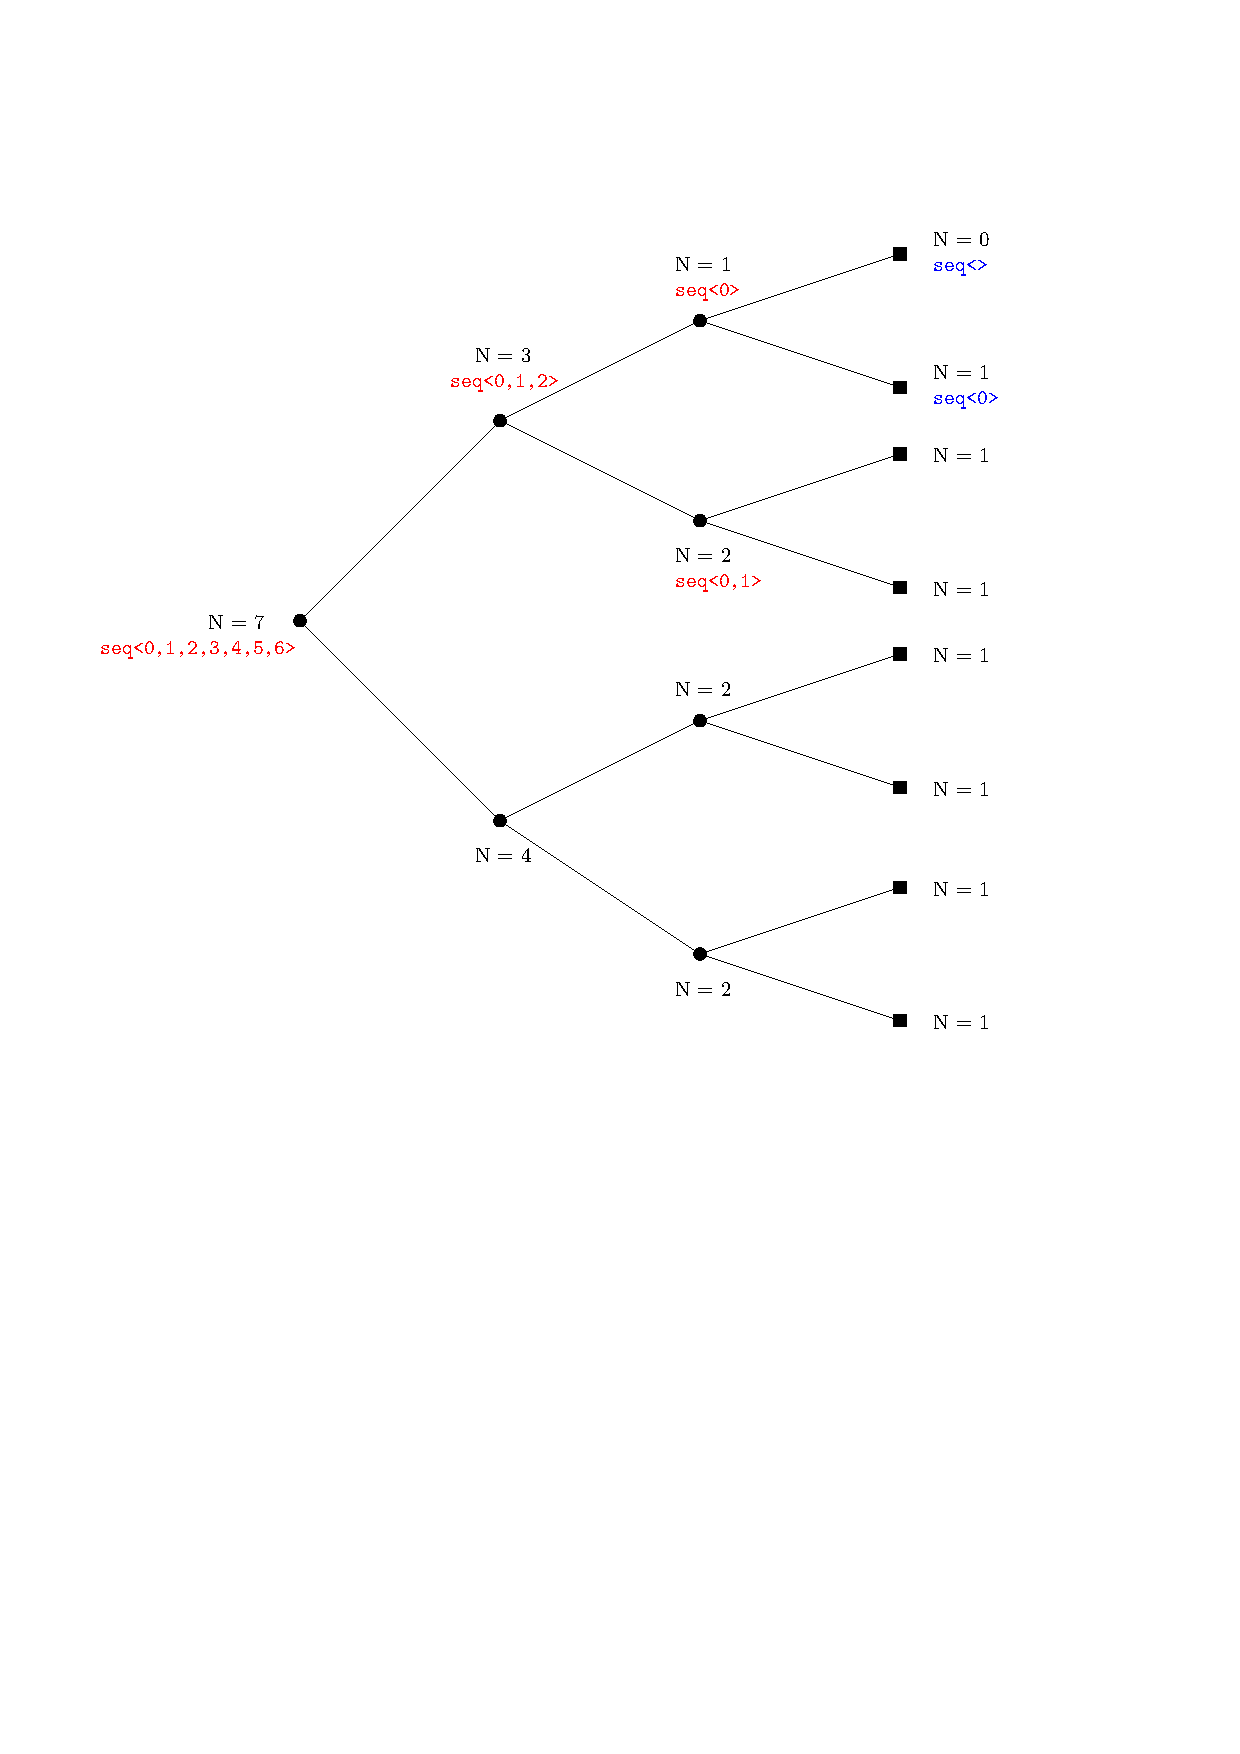
\includegraphics[width=0.99\textwidth]{logarithmic_seq}
      \end{figure}
    \end{column}%
  \end{columns}
\end{frame}


\begin{frame}[fragile]{Tinkering}
\begin{lstlisting}
template<int... I1, int... I2>
struct concat<seq<I1...>, seq<I2...> >
{
  static constexpr @\aftergroup\bluecolor@int _N1@\aftergroup\blackcolor@ = sizeof...(I1);
  using type = seq<I1..., (@\aftergroup\bluecolor@_N1@\aftergroup\blackcolor@ + I2)...>;
};
\end{lstlisting}

~

\begin{lstlisting}
using S = make_seq_t<5000>; // compile time: 4.045s
\end{lstlisting}
\end{frame}


\begin{frame}[fragile]{More tinkering}
\begin{lstlisting}
template<int... I1, int... I2>
struct concat<seq<I1...>, seq<I2...> >
{
  @\aftergroup\bluecolor@using _N1@\aftergroup\blackcolor@ = std::integral_constant<int, sizeof...(I1)>;
  using type = seq<I1..., (@\aftergroup\bluecolor@_N1()@\aftergroup\blackcolor@ + I2)...>;
};
\end{lstlisting}

~

\begin{lstlisting}
using S = make_seq_t<5000>; // compile time: 0.148s
\end{lstlisting}
\end{frame}


\section{Mapping indices}


\begin{frame}[fragile]{Storing data off the tree}
\begin{lstlisting}
auto evaluate(A &a, B &b)
{
  // (to be revisited)
  auto @\aftergroup\bluecolor@c0@\aftergroup\blackcolor@ = 4.2_f;
  auto @\aftergroup\bluecolor@c1@\aftergroup\blackcolor@ = rand();

  // build expression tree
  auto t0 = a * b;
  auto t1 = @\aftergroup\bluecolor@c0@\aftergroup\blackcolor@ + t0;
  auto t2 = @\aftergroup\bluecolor@c1@\aftergroup\blackcolor@ + t0;
  return t1 / t2;
}
\end{lstlisting}
\end{frame}


\begin{frame}[fragile]{Storing data off the tree}
  \begin{columns}[T] % align columns
    %% \begin{column}{0.3\textwidth}
    %% \end{column}%
    %% \hfill%
    \begin{column}{0.75\textwidth}
      \begin{figure}[H]
        \centering
        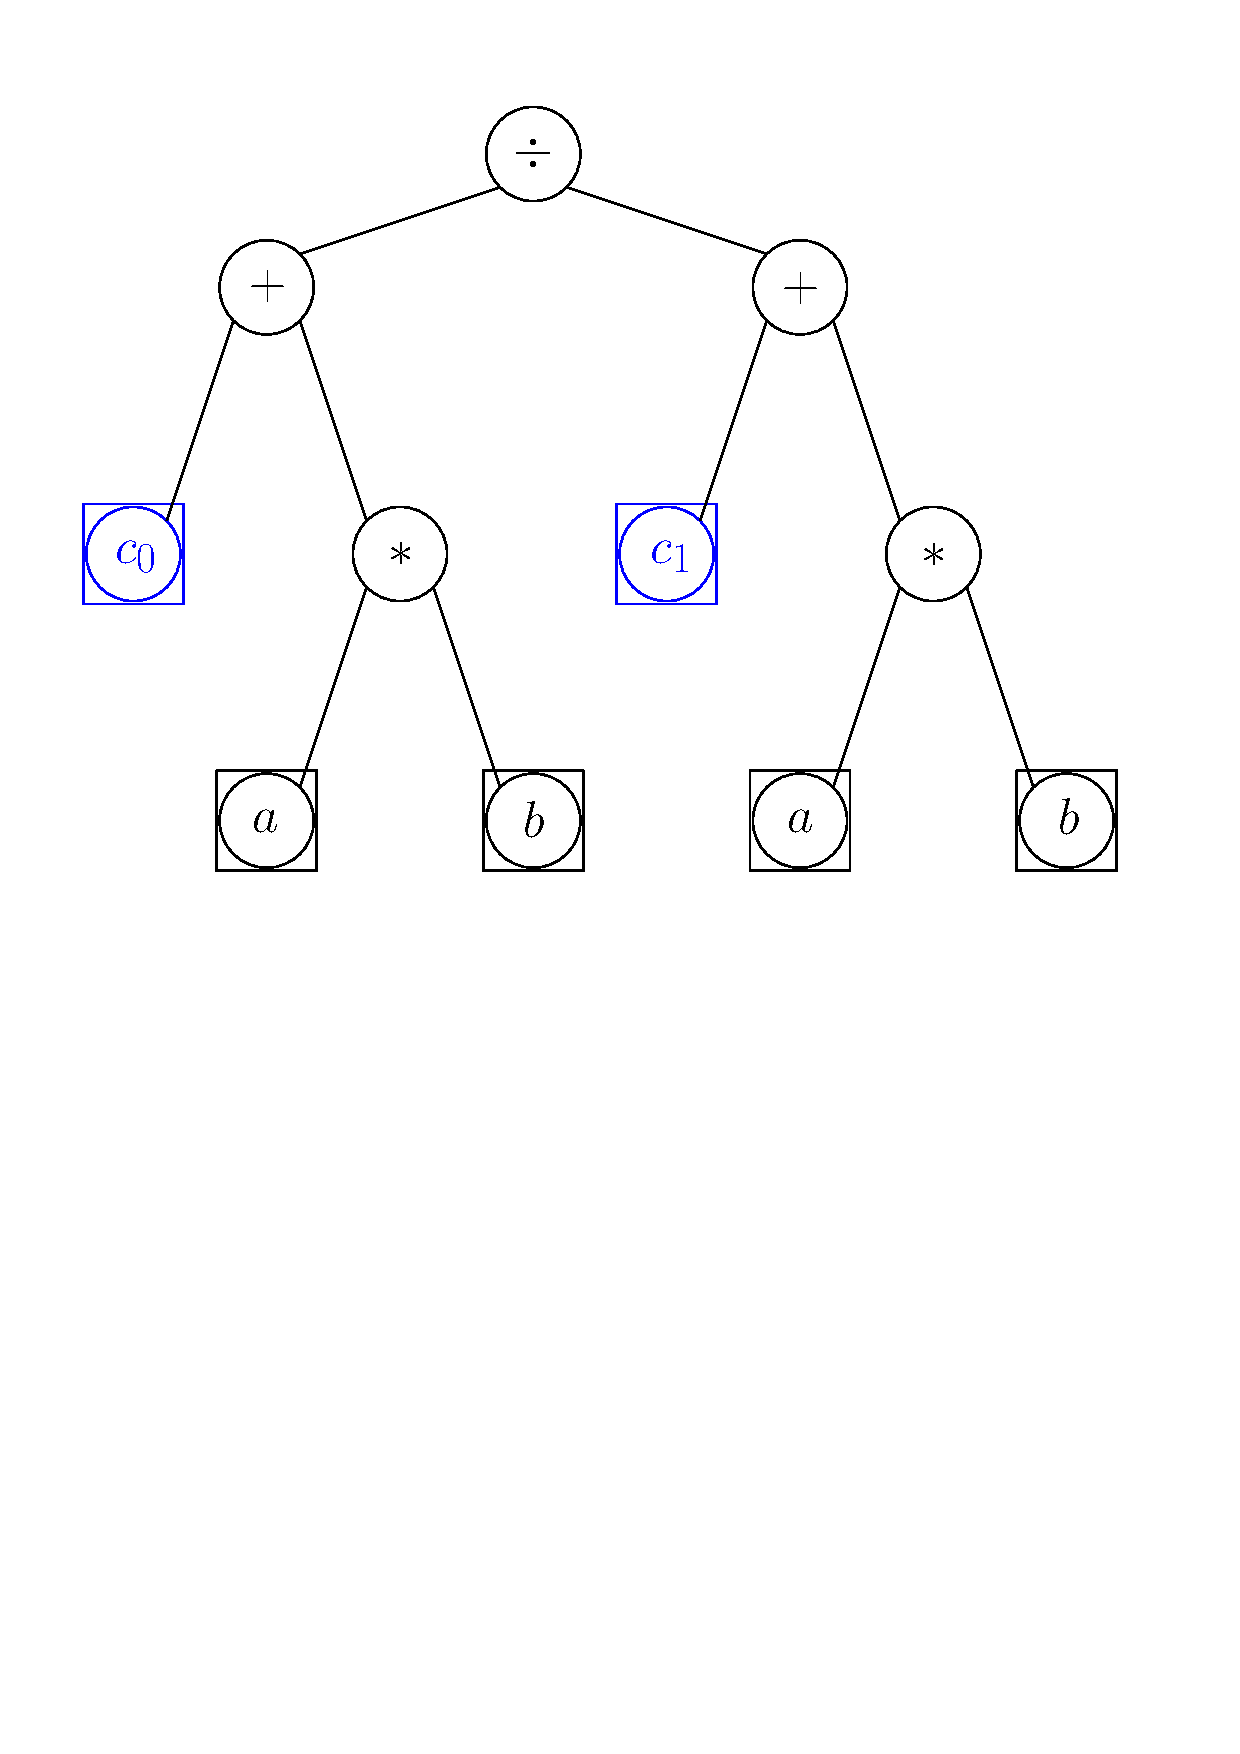
\includegraphics[width=0.99\textwidth]{fig_exprtree_cb}
      \end{figure}
    \end{column}%
  \end{columns}
\end{frame}


\begin{frame}[fragile]{Storing data off the tree}
With operator overloading
\begin{lstlisting}
  Binary<Div,
    Binary<Add, @\aftergroup\bluecolor@C0@\aftergroup\blackcolor@,
      Binary<Mul, A, B> >
    Binary<Add, @\aftergroup\bluecolor@C1@\aftergroup\blackcolor@,
      Binary<Mul, A, B> > >
\end{lstlisting}

~

then flattening...
\begin{lstlisting}
 {Binary<Mul, A, B>,
  Binary<Add, @\aftergroup\bluecolor@C0@\aftergroup\blackcolor@, [...]>,
  Binary<Add, @\aftergroup\bluecolor@C1@\aftergroup\blackcolor@, [...]>,
  Binary<Div, [...], [...]>}
\end{lstlisting}
\end{frame}


\begin{frame}[fragile]{Mapping nodes to data}
Look-up of {\color{blue}\texttt{C0}} and {\color{blue}\texttt{C1}} required
\begin{lstlisting}
  L = {A,                                //  0
       B,                                //  1
       Binary<Mul, A, B>,                //  2
       Binary<Add, @\aftergroup\bluecolor@C0@\aftergroup\blackcolor@, [...]>,           //  3  <--
       Binary<Add, @\aftergroup\bluecolor@C1@\aftergroup\blackcolor@, [...]>,           //  4  <--
       Binary<Div, [...], [...]>}        //  5
\end{lstlisting}
\begin{lstlisting}
  array<float, 2> @\aftergroup\bluecolor@c@\aftergroup\blackcolor@ = {4.2, rand()};
\end{lstlisting}

~

Indices of constants in `\texttt{L}'
\begin{lstlisting}
  IC = {3, 4}
\end{lstlisting}

~

Map elements in `\texttt{L}' to storage offsets
\begin{lstlisting}
  DC = {2, 2, 2, 0, 1, 2}
\end{lstlisting}
\end{frame}


\begin{frame}[fragile]{Dual function}
\begin{lstlisting}
// homework
//----------
DC_SIZE = 6     \
                 --- @\aftergroup\bluecolor@Dual@\aftergroup\blackcolor@ --->    DC = {2, 2, 2, 0, 1, 2}
IC = {3, 4}     /                       @\aftergroup\graycolor@0  1  2  3  4  5@\aftergroup\blackcolor@
\end{lstlisting}

~

\begin{lstlisting}
// step 1: index the input
IC_MAP = {{3, 0}, {4, 1}}
\end{lstlisting}
\end{frame}


\begin{frame}[plain]
  \begin{columns}[T] % align columns
    \begin{column}{0.5\textwidth}
      \begin{figure}[H]
        \centering
        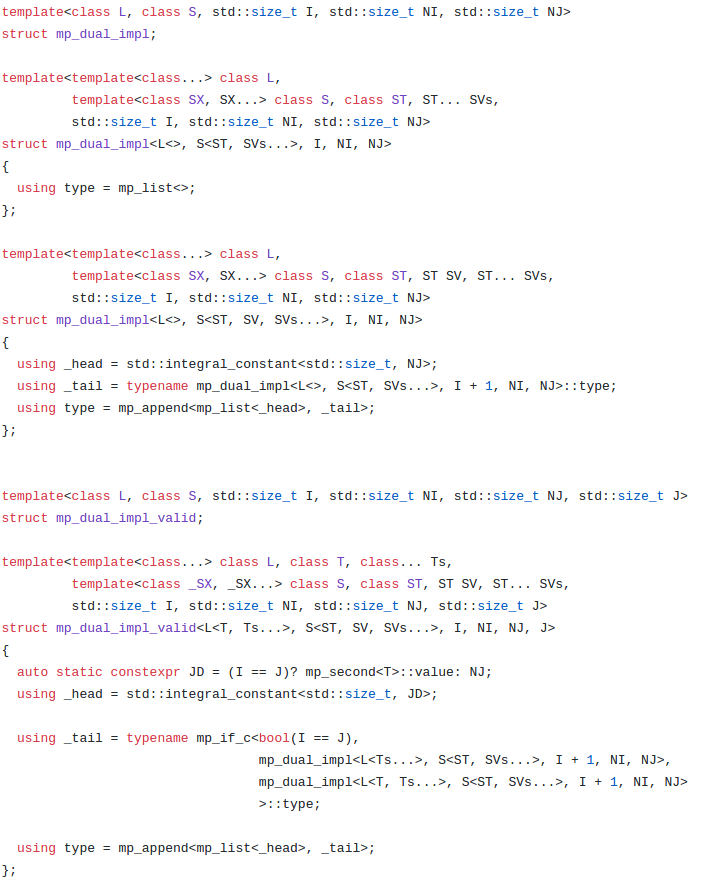
\includegraphics[width=0.99\textwidth]{dual_1}
      \end{figure}
    \end{column}%
    \hfill%
    \begin{column}{0.5\textwidth}
      \begin{figure}[H]
        \centering
        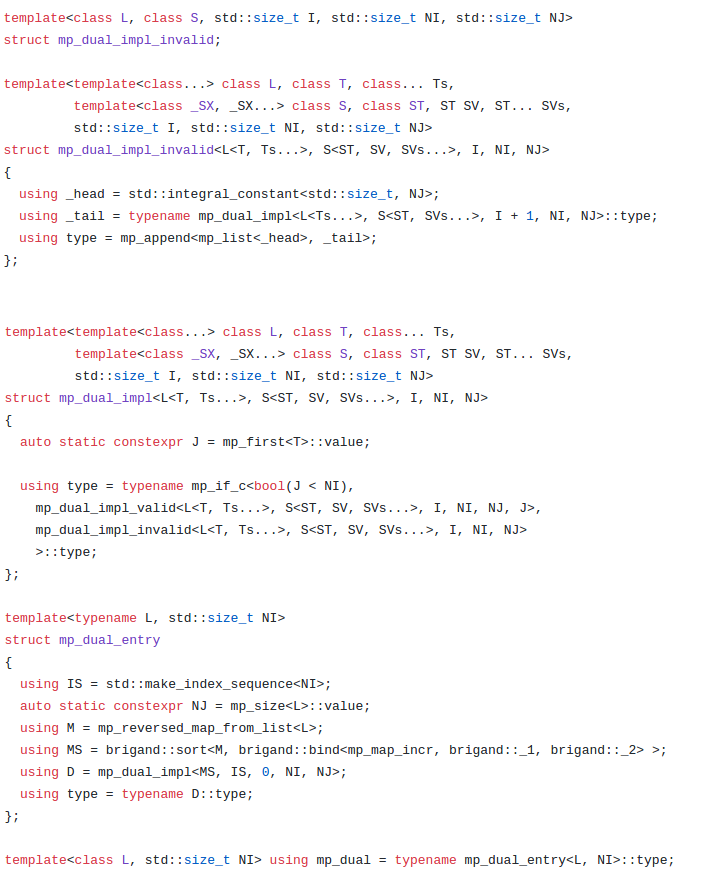
\includegraphics[width=0.99\textwidth]{dual_2}
      \end{figure}
    \end{column}%
  \end{columns}

\vspace{5mm}
\footnotesize{\texttt{github.com/DominicJones/snippets/blob/master/Cxx/mp\_functions.cpp}}
\end{frame}


\section{Four last things}


\begin{frame}[fragile]{Mutually exclusive?}
\begin{lstlisting}
auto constexpr @\aftergroup\bluecolor@list@\aftergroup\blackcolor@ = [](auto ...x)
{
  return [=](auto f){ return f(x...); };
};
\end{lstlisting}

~

\begin{lstlisting}
auto constexpr length = [](auto x)
{
  return x([](auto ...f){ return sizeof...(f); });
};
\end{lstlisting}

~

\begin{lstlisting}
auto constexpr n = length(@\aftergroup\bluecolor@list@\aftergroup\blackcolor@(true, 'c', 3.14));
\end{lstlisting}
\end{frame}


\begin{frame}[fragile]{\texttt{g++ demangle}}
\begin{lstlisting}[basicstyle=\tiny\ttfamily]
#include <cxxabi.h>

struct Demangle
{
  static std::string eval(char const * name)
  {
    int status(-4);
    char * realname;
    realname = abi::__cxa_demangle(name, 0, 0, &status);
    std::string result(realname);
    free(realname);
    return result;
  }
};

template<typename Expr_t>
std::string demangle(Expr_t const &expr)
{
  return Demangle::eval(typeid(expr).name());
}

template<typename Expr_t>
std::string demangle()
{
  return Demangle::eval(typeid(Expr_t).name());
}
\end{lstlisting}

\begin{lstlisting}[basicstyle=\tiny\ttfamily]
// very helpful
std::cout << demangle(complicated_type{}) << std::endl;
\end{lstlisting}
\end{frame}


\begin{frame}[fragile]{Low hanging fruit}
\begin{lstlisting}
// permit `auto' to resolve as `float'
template<auto V>
struct @\aftergroup\redcolor@_float@\aftergroup\blackcolor@
{
  constexpr operator auto() const { return V; }
};

// only interested in the type
auto constexpr c0 = 4.2@\aftergroup\redcolor@_f@\aftergroup\blackcolor@;
static_assert(c0 == @\aftergroup\redcolor@_float@\aftergroup\blackcolor@<4.2>{});
\end{lstlisting}

\vspace{5mm}
\footnotesize{D has had this for years...}\newline
\footnotesize{\texttt{dlang.org/spec/template.html}}
\end{frame}


\begin{frame}[fragile]{The third realm}
\begin{lstlisting}
@\aftergroup\graycolor@ 1234567@\aftergroup\bluecolor@8@\aftergroup\graycolor@9 123456789 12345
         10        20
1
2  // main.cpp
@\aftergroup\bluecolor@3@\aftergroup\graycolor@@\aftergroup\blackcolor@  auto @\aftergroup\bluecolor@c1@\aftergroup\blackcolor@ = rand();@\aftergroup\graycolor@
4@\aftergroup\blackcolor@  auto constexpr c1_loc = @\aftergroup\redcolor@&@\aftergroup\blackcolor@c1;@\aftergroup\graycolor@
\end{lstlisting}

~

\begin{lstlisting}
// reflect location
@\aftergroup\redcolor@&@\aftergroup\blackcolor@c1 := @\aftergroup\redcolor@hash(row, column, filename)@\aftergroup\blackcolor@
    := @\aftergroup\redcolor@hash(@\aftergroup\bluecolor@3@\aftergroup\redcolor@, @\aftergroup\bluecolor@8@\aftergroup\redcolor@, @\aftergroup\greencolor@`$PATH/main.cpp`@\aftergroup\redcolor@)
\end{lstlisting}

\vspace{5mm}
\footnotesize{A rough draft on it...}\newline
\footnotesize{\texttt{github.com/DominicJones/articles/blob/master/cxx-sg7-varid}}
\end{frame}


\begin{frame}[plain]
  \titlepage
\end{frame}


\end{document}
